%%%%%%%%%%%%%%%%%%%%%%%%%%%%%%%%%%%%%%%%%%%%%%%%%%
%% Authors :    Giovanni Arcari                 %%
%%              Maria Bronzova                  %%
%%              Luca Sardi                      %%
%%              Spencer Sharp                   %%
%%                                              %%
%% Supervisor : Andreas Apostolatos             %%
%%											  	%%
%% e-mail : andreas.apostolatos@tum.de		   	%%
%%											  	%%
%% 06_Problem.tex					  	   	 	%%
%%											  	%%
%%%%%%%%%%%%%%%%%%%%%%%%%%%%%%%%%%%%%%%%%%%%%%%%%%
\section{PROBLEM CASE}

In order to show the capabilities of the code which has been developed, how results are shown, and how to interpret a sensitivity analysis, an example is provided.\\[3pt]
It's important to notice that the following constitutes just a single application of the code, which - as explained later - is able to perform calculations on any kind of arbitrary structure that the user sets up through GiD. In this particular case, the aim is to show a simple case, whose behavior can be found intuitive by those readers who have even just a basic understanding of structural mechanics.

\subsection{Sensitivity analysis on a cantilever beam}
\subsubsection{Geometry and boundary conditions}
As explained, the case for the analysis example is chosen to be intuitive and broadly known. For this reason, a cantilever beam has been chosen. As illustrated in Figure \ref{cantileverBeam:BCs}, the left edge of the beam is fixed; horizontal and vertical displacements are constrained, as well as the rotations.\\
\begin{figure}[ht]
\centering
  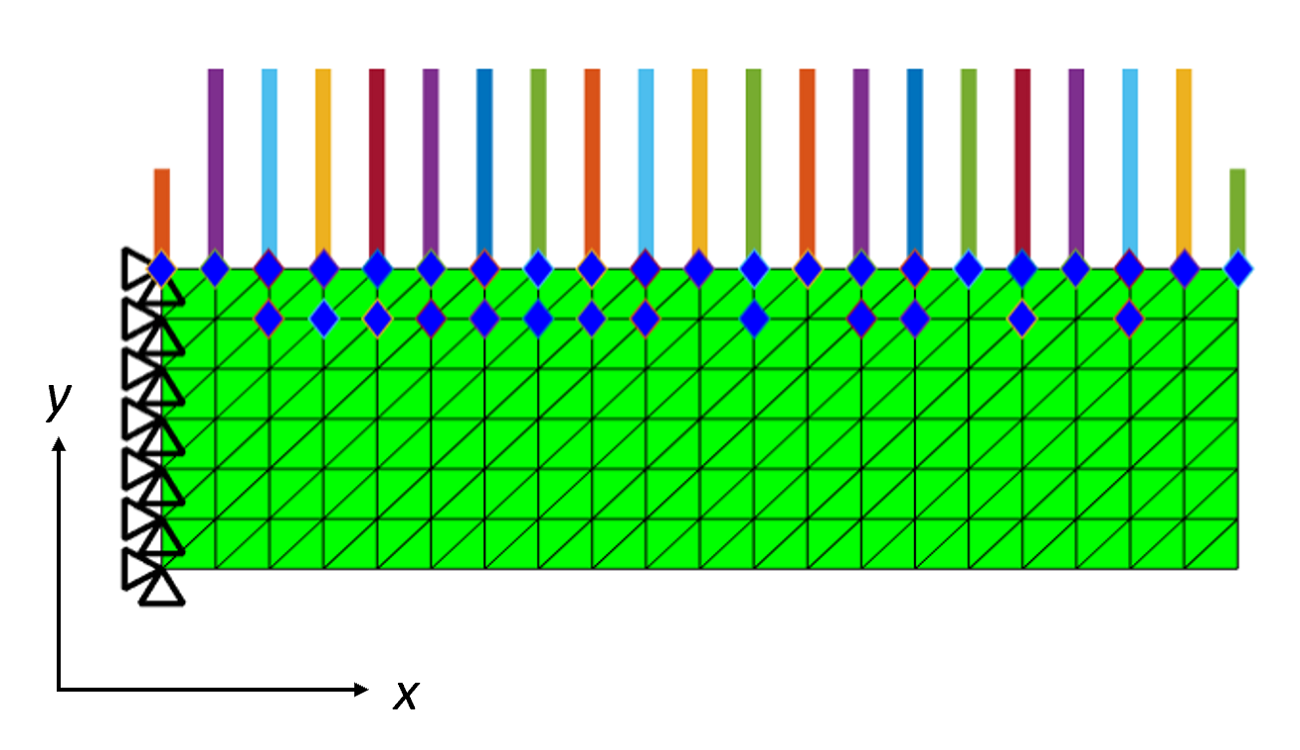
\includegraphics[width=100mm]{images/cantileverBeamBCs.png}
  \caption{Boundary conditions for cantilever beam}
  \label{cantileverBeam:BCs}
\end{figure} \\
The simulated beam has a width of $1.75m$ and a height of $0.5m$.
The slenderness, defined in this case by the ratio between the major and the minor dimensions, is  $3.5$. 
\subsubsection{Material properties}
In this example, the beam is made of steel.\\[3pt]
Accordingly, the following material properties have been applied to the model: 
\begin{itemize}
\item Young's modulus: $E = 210 GPa$
\item Poisson's ratio: $\nu = 0.33$
\item Thermal expansion coefficient: $\alpha = 0$
%\item Density: $\rho = has it been considered?$ MAYBE ADD LATER
\item Plane stress
\item Linear elastic isotropic
\end{itemize}
\subsubsection{Loads}
Loads have been applied on the upper edge, a constant pressure $p = 1x10^{3} \frac{N}{m}$ in the negative y-direction is considered.
\subsubsection{Mesh}
GiD provides the user with various options for mesh generation. For the purpose of this example, a simple structured mesh consisting of linear triangular elements has been created using GiD's automatic mesh generation function. See Figure \ref{cantileverBeam:mesh} below. \\[3pt]
According to finite element literature \cite{FEM_felippa}, the number of elements should be the smallest which can capture the behavior of the structure to a sufficient level of accuracy, in order achieve a balance of satisfying results and reasonable computational effort. \\[3pt]
As noticed by running different cases, it is possible to get a non-distorted mesh by choosing this length as an integer fraction of the beam dimension. Since the structure is rectangular, it is possible to get a uniform mesh, where all triangles have the same shape and size, and no distortion occurs. \\[3pt]
\begin{figure}[ht]
\centering
  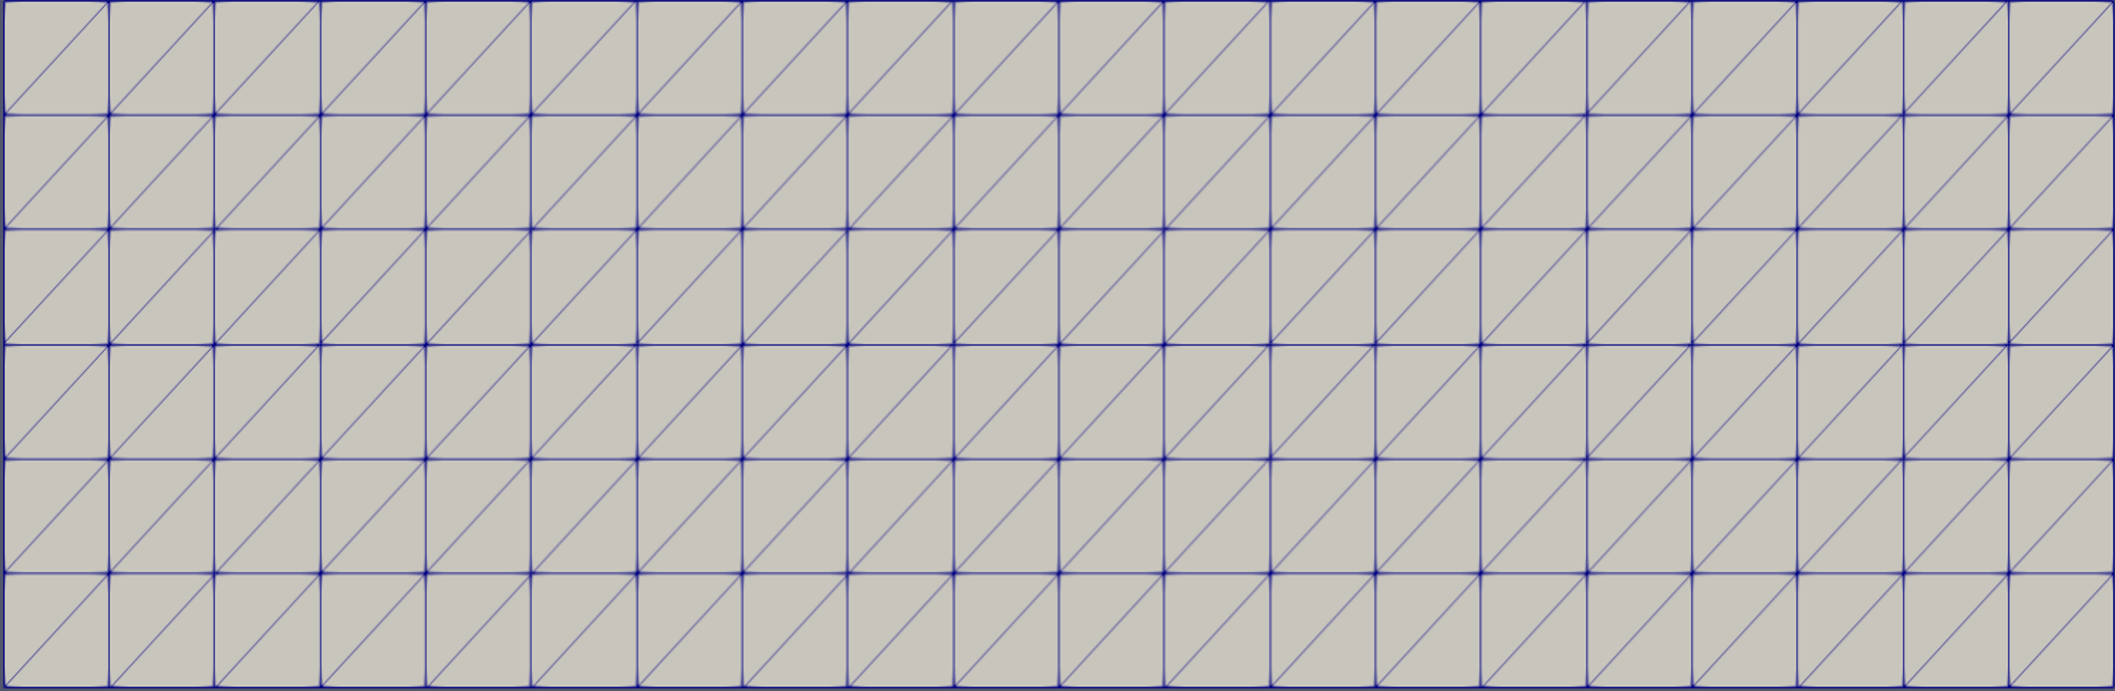
\includegraphics[width=100mm]{images/mesh.png}
  \caption{Generated mesh for cantilever beam}
  \label{cantileverBeam:mesh}
\end{figure}
In this case, six elements are chosen in the vertical direction, and twenty in the horizontal direction. Since the mesh is triangular, this leads to a total of 240 elements. It could be argued that the mesh is even too fine for the problem case; however, it's useful to keep in mind that the computational time using a common laptop was short enough to that no significant advantage could be had by the usage of a coarser mesh. Therefore, the mesh is kept as shown in the figure.\\[3pt]
For the purpose of numerical integration over both the domain and the boundary, the number of Gauss points must be specified. GiD defaults to assuming one Gauss point per element, which is what was used in this example.\\[3pt]


